\documentclass{article}
\usepackage{amsmath} % Required for mathematical symbols and fonts
\newcommand{\abs}[1]{\left|#1\right|}
\usepackage{graphicx} % Required for inserting images
\usepackage{tikz}
\usepackage{amssymb} % Required for additional mathematical symbols
\usepackage{amsthm}

\theoremstyle{remark}
\newtheorem*{remark}{Remark}
\usepackage[T1]{fontenc}
\usepackage{lmodern}

\title{Convergence of sequences sheet I}
\author{Gallo Tenis / to A Mathematical Room}

\begin{document}

\maketitle

\begin{center}
    \textit{Problems on convergence of sequences and fundamental real number properties from the books Terence Tao's ``Analysis I'',
    Michael Spivak's ``Calculus'' and Bartle R.G. ``Introduction to Real Analysis'' plus some of my own.
    } 
\end{center}
\section{Real numbers}
    \subsection*{Cauchy Sequences}
    \begin{enumerate}
        \item \textbf{(Cauchy sequences are bounded)}. Every Cauchy sequence $(a_n)_{n=1}^{\infty}$
        is bounded.\\
        $\textbf{Solution.}$ Suppose for the sake of contradiction that the sequence $(a_n)_{n=1}^{\infty}$
        is not bounded.
        That is, for any rational number $M\geq 0$, there exists some natural number $n_M \geq 1$ such that
        \begin{center}
            $\displaystyle \vert a_{n_M} \vert > M$.
        \end{center}
        Since $(a_n)$ is a Cauchy sequence, we have that for any $\varepsilon > 0$,
        there exists a natural number $n_{\varepsilon} \geq 1$ such that for any $n,m \geq n_{\varepsilon}$
        $\left\lvert a_n - a_m \right\rvert \leq \varepsilon$.
        This implies that 
        \begin{center}
            $-\varepsilon+a_m \leq a_n \leq \varepsilon + a_m$.\\
        \end{center}        
        The finite sequence $(a_n)_{n=1}^{n_M}$ is bounded, meaning that 
        there exists some rational number $M' \geq 0$ such that $\vert a_n \vert \leq M'$
        for any $1\leq n \leq n_M$. But clearly as the starting inequality shows, this sequence
        cannot be bounded by $\min (M, M')$. In fact, any finite sequence $(a_n)_{n\geq n_M}$ 
        cannot be bounded by $\min (M, M')$.

        Let $\varepsilon \leq \min (M, M')$. Then, for some $n_M \geq n_{\varepsilon} \geq 1$, take $n, m \geq n_{\varepsilon}$
        \begin{center}
            $\varepsilon \leq a_n \leq -\varepsilon$
        \end{center}
        But by the inequality given by the fact that $(a_n)$ is a Cauchy sequence we have (adding both inequalities):
        \begin{center}
            $a_m \leq 2a_n \leq a_m$
        \end{center}
        Hence $a_m = 2a_n$, which is then greater than $\varepsilon$.
        Thus:
        \begin{center}
            $\vert a_n - a_m \vert = \vert a_n\vert \geq \varepsilon$.
        \end{center}
        So it shows that $(a_n)$ is not a Cauchy sequence, a contradiction.
        \begin{flushright}
            \qed
        \end{flushright}
        \item Show that if \( (a_n)_{n=1}^{\infty} \) and \( (b_n)_{n=1}^{\infty} \) are 
        equivalent sequences of rationals, then \( (a_n)_{n=1}^{\infty} \) is a Cauchy sequence if and only if \( (b_n)_{n=1}^{\infty} \) is a Cauchy sequence.\\
        $\textbf{Solution.}$
        Assume that $(a_n)$ is a Cauchy sequence.
        Then, for any $\varepsilon/2 > 0$, there exists
        a natural number $n_{\epsilon}$ such that for any consecutives $n,m \geq n_{\varepsilon}$:
        $\vert a_n - a_m \vert \leq \varepsilon/2$. Since both $(a_n), (b_n)$ are equivalent
        there exists an $m_{\varepsilon}$ such that $\vert a_n - b_n \vert \leq \varepsilon/2$ for any
        $n \geq m_{\varepsilon}$.
        Let $M := \max(n_{\varepsilon}, m_{\varepsilon})$. Fixing this $M$ we get that 
        both properties for the sequences hold for any $n,m \geq M$ and
        we are allowed to do the following derivation:
        \begin{center}
            $\vert b_n - b_m\vert = \vert (a_n + b_n) - (a_m + b_m)\vert
            = \vert (a_n - b_n) + (a_m - b_m)\vert \leq \vert a_n - b_n \vert + \vert a_m - b_m\vert
            \leq 2\varepsilon/2 = \varepsilon$.
        \end{center}
        Which shows that $(b_n)$ is a Cauchy sequence.
        The converse implication has the same derivation, replacing $(a_n)$ with $(b_n)$.
        \begin{flushright}
            \qed
        \end{flushright}

        \item Let \( \varepsilon > 0 \). Show that if \( (a_n)_{n=1}^{\infty} \) and \( (b_n)_{n=1}^{\infty} \) are eventually \( \varepsilon \)-close, then \( (a_n)_{n=1}^{\infty} \) is bounded if and only if \( (b_n)_{n=1}^{\infty} \) is bounded.\\
        $\textbf{First Solution.}$ 
        Assume that $(a_n)$ is bounded. Thus,
        \begin{center}
            $\vert a_n \vert \leq M$
        \end{center}
        For any $n \in \mathbb{N}$ and some rational number $M \geq 0$.
        Since $(a_n)$ and $(b_n)$ are equivalent eventually $\varepsilon-close$,
        for any $\varepsilon \geq 0$, there exists some integer $N\geq 1$, such that 
        \begin{center}
            $\vert a_n - b_n \vert \leq \varepsilon$ for every $n \geq N$.
        \end{center}
        This implies that
        \begin{center}
            $b_n \leq \varepsilon + a_n \leq \varepsilon + M$.
        \end{center}
        This does not yet imply that $b_n$ is bounded, since we have not checked what happens for the previous terms before $N$.
        Note that the finite sequence $(b_n)_{n\leq m}$ is bounded by, say, $M' := \max{(b_n)_{n\leq m}}$.
        So letting $m = N$ we get that the sequence $(b_n)_{n\leq N}$ is bounded by $M'$
        and $(b_n)_{n\geq N+1}$ is bounded by $\varepsilon + M$.
        
        Finally, let $K := \max(M',M+\varepsilon)$, this works as an upper bound of $(b_n)$.

        $\textbf{Second Solution.}$
        This solution uses the least upper bound property, which is not yet seen in the last problems.
        
        Let $L$ be the bound of $(a_n)$.
        Consider $M_N := \max{(a_n)_{n\leq N}}$, and $M'_N := \max{(b_n)_{n\leq N}}$ to be the upper bounds for finite truncations
        of $(a_n)$ and $(b_n)$. We notice that $M_N \leq M_{N+1}$ and $M'_N \leq M'_{N+1}$.

        Let $(K_N) := \max{(M_N, M'_N)}$ be a sequence. We claim that $K_N$ converges.
        Sort by values the sequences $(a_n)$ and $(b_n)$, we get that the new sequence $(a'_n)$ converges, since
        it is increasing and bounded, and it converges to $\sup (a'_n) \leq L$.

        Since $(a_n)$ and $(b_n)$ are equivalent, then for each $\varepsilon \geq 0$, there exists some natural number
        $N$ such that for any $n \geq N$:
        \begin{center}
            $\vert a_n - b_n \vert \leq \varepsilon$.
        \end{center}
        This means that $b_n \leq \varepsilon + a_n$ in the original sequence.
        We claim that, in the new sequence, the distance $\vert a'_n - b'_n \vert$ decreases or stabilizes (converges).

        We certainly cannot yet assume that from a certain point on after, the difference will still be decreasing. This is OK,
        since we aim to get a stable difference in order to get a bound for $(b'_n)$.

        Recalling the first paragraph, let $m \geq 1$ be an integer, we have that for some $N$,
        every $n \geq m$ will satisfy
        \begin{center}
            $L \geq a'_n \geq M_N$.
        \end{center}
        Similarly, for $(b'_n)$, for some $m'\geq 1$, there exists some $N'$ such that for every $n \geq m'$
        \begin{center}
            $L + \varepsilon \geq b'_n \geq M'_{N'}$ (since $b_n \leq \varepsilon + a_n$).
        \end{center}
        So, letting $m_0 := \max(m, m')$, we get these both properties holding simultaneosly.
        Hence:
        \begin{center}
            $\varepsilon \geq b'_n - a'_n \geq M'_{N'} - M_N$ (subtracting inequalities)
        \end{center}
        
        So far we get that $\varepsilon \geq b'_n - a'_n$. This means that for any $\varepsilon \geq 0$, 
        $b'_n \leq \varepsilon + \sup(a'_n)$ for any $n \geq m_0$.
        Thus $\sup (b'_n) \leq \sup(a'_n) + \varepsilon$.

        (Can we end up proving the first claim for $K_N$? I do not think it is needed, as it is equivalent $-$I believe$-$ to the last thing (that $b'_n$ is bounded).
        But it would be an interesting approach.)
        \begin{flushleft}
            \qed
        \end{flushleft}
        \item \textbf{(Formal limits are well-defined).} Let \( x =
        \lim_{n \to \infty} a_n \), \( y = \lim_{n \to \infty} b_n \), and \( z = \lim_{n \to \infty} c_n \) be real numbers.
        Then, with the definition of equality for real numbers, we have
        \( x = x \). Also, if \( x = y \), then \( y = x \). Finally, if \( x = y \) and \( y = z \), then
        \( x = z \). \\
        $\textbf{Proof.}$ For the case $x = x$, we have to prove that for the Cauchy sequence $(a_n)$, 
        $a_n$ is eventually $\varepsilon-close$ to itself, hence, take $\varepsilon \geq 0$, take any $N \geq 1$, for any $n \geq N$ we 
        will have:
        \begin{center}
            $\vert a_n - a_n \vert = 0 \leq \varepsilon$
        \end{center}
        So it shows that this sequence is equivalent to itself.
        The second case is also trivial, we get that
        \begin{center}
            $\vert a_n - b_n \vert = \vert b_n - a_n \vert \leq \varepsilon$
        \end{center}
        Given that $(a_n) \equiv (b_n)$.
        For the transitivity part, given that for any $\varepsilon/2 \geq 0$, there exist numbers $N, M\in \mathbb{N}$ such that
        \begin{center}
            $\vert a_n - b_n \vert \leq \varepsilon/2 \text{ for any }n\geq N$
        \end{center}
        \begin{center}
            $\vert b_n - c_n \vert \leq \varepsilon/2 \text{ for any }n\geq M$
        \end{center}
        taking $K := \max(N,M)$ both properties hold at the same time, then
        \begin{center}
            $\vert b_n - c_n \vert + \vert a_n - b_n \vert
            \leq \varepsilon \text{ for any }n\geq K$
        \end{center}
        Thus, by triangle inequality:
        \begin{center}
            $\vert b_n - c_n + a_n - b_n \vert
            = \vert a_n - c_n \vert \leq \varepsilon \text{ for any }n\geq K$
        \end{center}
        \begin{flushright}
            \qed
        \end{flushright}
        \item \textbf{(Multiplication is well-defined).} Let \( x =
        \lim_{n \to \infty} a_n \), \( y = \lim_{n \to \infty} b_n \), and \( x' = \lim_{n \to \infty} a'_n \) be real numbers.
        Then \( xy \) is also a real number. Furthermore, if \( x = x' \),
        then \( xy = x'y \).\\
        $\textbf{Proof.}$
        Since $(a_n)$ and $(b_n)$ are Cauchy sequences, for any $\varepsilon > 0$ there must exist an integer $N,M \geq 1$ such that 
        for any $n,m \geq K := \max(N,M)$
        \begin{center}
            $\displaystyle \vert a_n - a_m \vert \leq \varepsilon$ and $\displaystyle \vert b_n - b_m \vert \leq \varepsilon$.
        \end{center}
        So our goal is to show that 
        \begin{center}
            $\displaystyle \vert b_na_n - b_ma_m\vert \leq \varepsilon$.
        \end{center}
        We first note that $b_na_n - b_ma_m = (b_n-b_m)a_n + b_m(a_n-a_m)$, hence the following chain of inequalities will hold for any $n,m \geq K$
        \begin{center}
            $\displaystyle \vert (b_n-b_m)a_n + b_m(a_n-a_m)\vert \leq \vert (b_n-b_m) a_n\vert + \vert b_m(a_n-a_m) \vert$.
        \end{center}
        By problem 1, $(a_n)$ and $(b_n)$ are bounded, so there must exist a rational number $M \geq 0$ such that $\vert a_n\vert, \vert b_n\vert \leq M$ for any $n \geq 1$ (where we found $M$ as the maximum between the bounds of both sequence).
        This means that the former inequality is bounded by
        \begin{center}
            $\displaystyle M(\vert b_n-b_m\vert + \vert a_n - a_m \vert) \leq M\varepsilon$.
        \end{center}
        This finishes up our proof as $M\varepsilon > 0 \iff \varepsilon > 0$.
        The next part of the problem is similar, we use the same identity as in this one, let $x' = \lim_{n\to\infty}a'_n$. The goal is to show that 
        \begin{center}
            $\displaystyle \vert (b_na_n - b_ma_m) - (b_na'_n - b_ma'_m) \vert \leq \varepsilon$,
        \end{center}
        as we want them to be equivalent sequences.
        Hence,
        \begin{center}
            $\displaystyle \vert (b_n-b_m)a_n + b_m(a_n-a_m) - ((b_n-b_m)a'_n + b_m(a'_n-a'_m))\vert$
        \end{center}
        \begin{center}
            $\displaystyle \leq \vert (M(b_n-b_m) + M(a_n-a_m)) - ((b_n-b_m)a'_n + b_m(a'_n-a'_m))\vert$
        \end{center}
        \begin{center}
            $\displaystyle = \vert (M(b_n-b_m) - M(a_n-a_m)) + ((b_n-b_m)a'_n - b_m(a'_n-a'_m)) \vert $  
        \end{center}
        \begin{center}
            $\displaystyle \leq M\vert (b_n-b_m) - (a_n-a_m)\vert + M\vert ((b_n-b_m) - (a'_n-a'_m)) \vert$  
        \end{center}
        \begin{center}
            $\displaystyle \leq 2M\varepsilon$ (since $\varepsilon - (a_n-a_m) > 0$).
        \end{center}
        \begin{flushright}
            \qed
        \end{flushright}

        \item Let \( a \) and \( b \) be rational numbers. Show that \( a = b \) if and only if 
        \( \lim_{n \to \infty} a = \lim_{n \to \infty} b \) (i.e., the Cauchy sequences \( a, a, a, a, \dots \) and \( b, b, b, b, \dots \) are equivalent if and only if \( a = b \)).\\
        $\textbf{Solution.}$
        We claim that for any $a, b$ rational numbers, then $\left\lvert a-b\right\rvert \leq \varepsilon$ for any $\varepsilon \geq 0$ if and only
        if $a = b$. To prove this claim assume for the sake of contradiction that if 
        $\left\lvert a-b\right\rvert \leq \varepsilon$ for any $\varepsilon \geq 0$ then $a \neq b$.
        Then without loss of generality assume $a > b$. Hence $\left\lvert a-b\right\rvert = a-b$. Then, if we take $\varepsilon_0 = 0$,
        $a - b = 0$, which implies that $a = b$.
        Conversely, if $a=b$, then $\left\lvert a-b\right\rvert = \left\lvert 0\right\rvert = 0$
        which is, by hypothesis, true.\\
        Then, let $a = b$. Suppose for the sake of contradiction that $\lim_{n\to \infty}a_n \neq \lim_{n\to \infty}b_n$.
        So there must exist some $\varepsilon_0 \geq 0$ such that for any $N \geq 1: \left\lvert a_n - b_n \right\rvert > \varepsilon_0$ for some
        values of $n \geq N$. Fixing this $n$ we get that $\left\lvert a_n - b_n \right\rvert = \left\lvert a - a \right\rvert = 0 > \varepsilon_0$,
        a contradiction, since $\varepsilon_0 > 0$.\\
        Conversely, suppose that given two equal real numbers $\lim_{n \to \infty} a_n$, $\lim_{n \to \infty} b_n$
        such that $a_n = a, b_n = b$ for any $n \geq 1$, implies that $a \neq b$.
        Since $\lim_{n \to \infty} a_n$, $\lim_{n \to \infty} b_n$ both sequences $(a_n)$ and $(b_n)$ are equivalent.
        Hence, for any positive number $\varepsilon \geq 0$ there exists an $N$ such that:
        \begin{center}
            $\left\lvert a-b\right\rvert \leq \varepsilon$
        \end{center}
        for every $n \geq N$. Since $a$ and $b$ do not depend in the choice
        of $N$, by the last claim, $a = b$.
        \begin{flushright}
            \qed
        \end{flushright}

        \item Show that \( \lim_{n \to \infty} \frac{1}{n} = 0 \).\\
        $\textbf{Solution.}$
        First we show that this sequence is Cauchy.
        We have to show that, for any $\varepsilon > 0$ there exists some integer $N \geq 1$ such that for any $n,m \geq N$
        \begin{center}
            $\displaystyle \abs{\frac{1}{n} - \frac{1}{m}} \leq \varepsilon$.
        \end{center}
        By Archimedean property, we can find
        \begin{center}
            $\displaystyle \varepsilon/2 > \frac{1}{M}$
        \end{center}
        where $M$ is a positive integer, hence 
        \begin{center}
            $\displaystyle M > 2/\varepsilon$.
        \end{center}
        So for $n,m \geq M$
        \begin{center}
            $\displaystyle \frac{1}{m}, \frac{1}{n} < \varepsilon/2$.
        \end{center}
        And note that
        \begin{center}
            $\displaystyle \abs{\frac{1}{n} - \frac{1}{m}} \leq \abs{\frac{1}{n} + \frac{1}{m}} \leq 2/M \leq \varepsilon$.
        \end{center}
        So this sequence is a Cauchy sequence, and it converges.
        
        Now we are in position to ask whether this sequence converges to a positive or negative real number. 
        And we claim that neither these cases are possible.
        To prove this claim suffices proving that this sequence is not bounded away from zero.

        We firstly note that the sequence $1/n$ cannot be negative.
        Suppose that there existed some rational number $c>0$ in which $1/n \geq c$ for any $n \geq 1$.
        This implies that if this were the case, $n \leq c$.
        By Archimedean property we can find some $N \geq 1$ in which 
        \begin{center}
            $\displaystyle \frac{1}{n} < Nc$ 
        \end{center}
        So suffices letting $a_{Nn} = 1/{Nn}$ to show that $a_n < c$.
        A more rudimentary method for this last part would be noting that $c := p/q$ with $p,q$ positive integers,
        then one can let $n = q$ so $a_q < c$.
        \begin{flushright}
            \qed
        \end{flushright}

        \item Let \( (a_n)_{n=0}^{\infty} \) be a sequence of rational numbers which is bounded. 
        Let \( (b_n)_{n=0}^{\infty} \) be another sequence of rational numbers which is equivalent to \( (a_n)_{n=0}^{\infty} \). 
        Show that \( (b_n)_{n=0}^{\infty} \) is also bounded.\\
        $\textbf{Solution.}$
        If one does not want to use problem 3, one can proceed as follows.
        Let $K/2 \in \mathbb{R}$ be a bound for $(a_n)$, this means that for any $n\in \mathbb{N}$
        \begin{center}
            $\vert a_n\vert \leq K/2$
        \end{center}
        As $(b_n)$ is equivalent to $(a_n)$, then for any $\varepsilon \geq 0$, there exist some $N\geq 1$ such that
        for every $n \geq N$:
        \begin{center}
            $\vert a_n - b_n \vert \leq \varepsilon$
        \end{center}
        This implies that 
        \begin{center}
            $b_n \leq \varepsilon + a_n$ for any $n \geq N$.
        \end{center}
        Let $\varepsilon = K/2$, this implies that for any $n \geq N_{K/2}$
        \begin{center}
            $b_n \leq K/2 + a_n \leq K/2 + K/2 = K$.
        \end{center}
        \begin{center}
            $b_n \geq -K/2 + a_n \geq 0$.
        \end{center}
        This, although, does not yet determines an absolute bound, we can choose a bound such as
        $M = \max(K, \max(b_n)_{n\leq N_K})$, since $(b_n)_{n\leq N_K}$ is bounded.
        Thus:
        \begin{center}
            $-M \leq 0 \leq b_n \leq M$
        \end{center}
        This means that $\vert b_n \vert \leq M$ for any integer $n \geq 1$.
        \begin{flushleft}
            \qed
        \end{flushleft}
        
        \item \textbf{(Basic properties of positive reals).} For every real number \( x \), exactly one of the following three statements is true: (a) \( x \) is zero; (b) \( x \) is positive; (c) \( x \) is negative. 
        A real number \( x \) is negative if and only if \( -x \) is positive. If \( x \) and \( y \) are positive, then so are \( x + y \) and \( xy \).\\
        $\textbf{Solution.}$
        (a) Suppose, for the sake of contradiction, that a number can be both zero and positive.
        Let $x := \lim_{n\to \infty}a_n$, $x > 0$ and $0 := \lim_{n\to\infty}0_n$. 
        
        This means that $(a_n)$ is equivalent to $(0_n)$, thus, for any $\varepsilon \geq 0$, there
        exists an $N$ such that for any $n\geq N$:
        \begin{center}
            $\vert a_n \vert \leq \varepsilon$
        \end{center}
        By definition of real number, we know that there exists some lower bound $c \in \mathbb{Q}$, $c > 0$ such that 
        $a_n \geq c$ for any $n \geq 1$.
        Thus, let $\varepsilon = c$, this implies that $a_n \leq c$ for every $n \geq N_c$, which is a contradiction.

        (b) Now, suppose that a real number can be both negative and positive simultaneosly,
        let $x := \lim_{n \to \infty}a_n$, $x > 0$ and $y := \lim_{n \to \infty}b_n$, $y < 0$ be real numbers.
        Our assumption implies that $(a_n)$ and $(b_n)$ are equivalent. This means that for any $\varepsilon \geq 0$, there exists
        some $N \geq 1$ such that for any $n \geq N$,
        \begin{center}
            $\vert a_n - b_n \vert \leq \varepsilon$
        \end{center}
        By definition of negative real number, there exists a rational number $-c < 0$ such that
        $b_n \leq -c$. This implies that $b_n < 0$, furthermore, it implies that $b_n = -\vert b_n \vert$. Thus:
        \begin{center}
            $\vert a_n - b_n \vert = \vert a_n + \vert b_n \vert \vert \leq a_n + \vert b_n \vert \leq \varepsilon$.
        \end{center}
        This implies that 
        \begin{center}
            $a_n \leq \varepsilon + b_n$
        \end{center}
        Let $\varepsilon = c$, it follows that:
        \begin{center}
            $a_n \leq c + b_n \leq c + (-c) = 0$
        \end{center}
        This is absurd, since $a_n$ is a strictly positive real number.

        (c) Now, we are going to prove that if a real number $x \in \mathbb{R}$ is negative, then $-x$ is positive,
        and viceversa.

        For the direct implication, let $(a_n)$ be a negatively upperly bounded Cauchy sequence, $x := \lim_{n\to \infty}a_n$ will be a negative real number.
        
        Suppose, for the sake of contradiction, that the sequence $(-a_n)$ is not a positively lowerly bounded Cauchy sequence.
        If that were the case, then there must exist some $n_0 \geq 0$ such that $-a_{n_0} \leq 0$.
        This implies that $-a_{n_0} \leq -c$, where $-c \leq 0$.
        Hence $a_{n_0} \geq c$. This would imply that $(a_n)$ is not negatively upperly bounded, which is a contradiction, by our hypothesis.

        Now, we would like to verify that $\lim_{n\to\infty}a_n + \lim_{n\to\infty}(-a_n) = 0$,
        to do this we might prove that their absolute value is the same ``at the limit''.
        This is straightforward since $\vert a_n \vert = \vert -a_n \vert$.

        The converse implication is analogous.

        (d) We claim that if $x, y$ are both positive real numbers, then $x + y$ is positive.
        Suppose, for the sake of contradiction, that the sequence $(a + b)_n := (a_n + b_n)$ is not positively lowerly
        bounded, this would imply that there exists some $n_0 \geq 1$ such that $(a+b)_{n_0} \leq 0$, thus $a_{n_0}+b_{n_0} \leq 0$.
        This would imply that $a_{n_0}$ and $b_{n_0}$ are negative or zero, which is contradictory to our hypothesis.
        An analogous reasoning is used to prove the case $x \times y > 0$.

        \begin{flushleft}
            \qed
        \end{flushleft}
        \item Prove that given any two real numbers \( x < y \), 
        we can find a rational number \( q \) such that \( x < q < y \).\\
        $\textbf{Solution.}$
        We use the results proved in problem 11.

        Let $M$ be an integer such that $M \geq x > M-1$ and let $N$ be an integer such that $N - 1 < y \leq N$,
        then $N-1 \geq M-1$. Then, there exists an integer $K$ such that
        \begin{center}
            $N-1 \geq K \geq M-1$, thus $y > K \geq x$
        \end{center}
        Let $q := (K+M-1)/2$, we see that $K \leq q \leq M-1$.

        \begin{flushleft}
            \qed
        \end{flushleft}

        \item Show that for every real number \( x \) there is exactly one integer \( N \) such that 
        \( N \leq x < N + 1 \). (This integer \( N \) is called the integer part of \( x \), 
        and is sometimes denoted \( N = \lfloor x \rfloor \).)\\
        $\textbf{First Solution.}$ Suppose that there existed two positive integers $N, M$ such that 
        \begin{center}
            $N \leq x < N + 1$ and $M \leq x < M + 1$.
        \end{center}
        This would imply that 
        \begin{center}
            $N - M \leq 0 \leq N - M$.
        \end{center}
        This implies that $N = M$.

        For the existence part, without loss of generality, assume $x > 0$,
        this implies that $x$ has a decomposition in a positively lowerly bounded Cauchy sequence.
        Thus, there must exist a rational number $c > 0$ such that $a_n \geq c$ for any integer $n \geq 0$.
        Also, this sequence is upperly bounded by some rational $K \geq 0$.
        These two rationals are our first approximation to $N$:
        \begin{center}
            $c\leq a_n \leq K$.
        \end{center}
        As $c$, $K$ and $a_n$ are rational numbers, there must exist a natural number $N$ such that 
        \begin{center}
            $0 \leq c\leq a_n \leq K \leq N$
        \end{center}
        In fact, suppose $\vert c - a_n \vert \leq 1$, then the natural number $1$ will satisfy that
        $0\leq c \leq a_n \leq 1$, similarly with $a_n$ and $K$.
        
        Formarly speaking, as $(a_n)$ is a Cauchy sequence, let $\varepsilon \geq 0$,
        let $N_{\varepsilon}$ be a positive integer; for any $n \geq N_{\varepsilon}$
        \begin{center}
            $\vert a_n - a_m \vert \leq \varepsilon$
        \end{center}
        and 
        \begin{center}
            $\vert a_n - a_m \vert \leq \vert c - K \vert$
        \end{center}
        We determine $N$ by the following sequence of steps:\\
        1) Start with setting $N_0:=K$ and $N'_0 := c$,
        this is, $N_0$ is a rational upper bound of $(a_n)$ and $N'_0$ is a rational lower bound of $(a_n)$.
        Also set $\varepsilon = \vert c - N_0 \vert$. Then, since $(a_n)$ is a Cauchy sequence, there exists
        $N_{\varepsilon} \geq 1$ such that for any $n, m \geq N_{\varepsilon}$
        \begin{center}
            $\vert a_n - a_m \vert \leq \varepsilon = \vert N'_0 - N_0 \vert$.
        \end{center}
        2) Lowerly bound $N_0$ by an integer $N_1$. 
        Upperly bound $N'_0$ by an integer $N'_1$. 
        
        Set $\varepsilon = \vert N'_1 - N_1 \vert$.
        Do the same argument as for (1) and the result is 
        \begin{center}
            $\vert a_n - a_m \vert \leq \vert N'_1 - N_1\vert$.
        \end{center}

        3) While $\vert N'_i - N_i \vert \geq 1$ repeat step (2).

        At the end, we will get some $N_k > N'_k$ such that $1 = \vert N_k - N'_k\vert \geq \vert a_n - a_m \vert$.
        This implies that $N_k \geq \lim_{n\to \infty }a_n > N'_k$ or $N_k > \lim_{n\to \infty }a_n \geq N'_k$.
        One can show this last thing by seeing that the sequence $(a_{n+N_{\varepsilon}})$ is upperly bounded by $N_k$ and lowerly bounded by $N'_{k}$,
        this means that
        \begin{center}
            $N_k \geq a_m > N'_k$
        \end{center}
        thus 
        \begin{center}
            $N_k \geq \lim_{n \to \infty}a_{n+N_{\varepsilon}} > N'_k$.
        \end{center}
        Since $(a_n)$ and $(a_{n+N_{\varepsilon}})$ converge to the same limit, this concludes our proof.
        Note that since their difference is 1 by construction then $N_k = N'_k + 1$.

        $\textbf{Second Solution.}$
        For the existence part, let $S := \{n \in \mathbb{Z}: n \leq x\}$ and
        $S' := \{n \in \mathbb{Z}: n > x\}$. 
        We first claim that these sets are non-empty. Note that we still do not have the least upper bound property, but we can
        proceed by Archimedean property. Let $\varepsilon = 1$, then there exists a positive integer $M$ such that $M\varepsilon > x$,
        this integer is just $N+1$ (if it was $N$ it might occur that it were equal to $x$), this implies that $S' \neq \emptyset$.
        
        Now, for $S$, taking some positive integer $M$ that is less than a lower bound of $(a_n)$ suffices; bounding a rational by an integer is always possible.

        Thus, $S'$ has minimum and it is $N+1$, therefore $N \notin S'$. This implies that $N \leq x$, thus $N \in S$.
        We conclude that $N = \max(S)$.
        Thus: $N+1 > x \geq N$.
        \begin{flushright}
            \qed
        \end{flushright}
        \item Show that for any positive real number \( x > 0 \) there exists a positive integer \( N \) such that \( x > \frac{1}{N} > 0 \).\\
        $\textbf{First Solution.}$ By the last problem, we can find a minimal integral upper bound $M$ for $x$ such that
        \begin{center}
            $M > x \geq M-1$.
        \end{center}
        Also, we can find a rational number $q = m/n$, with $0 \leq n+1 < m$ such that 
        \begin{center}
            $M > m/n \geq x$ and $x \geq (m-n)/n$.
        \end{center}
        In particular,
        \begin{center}
            $x > (m-n-1)/n$.
        \end{center}
        Let $N := n$, this results in:
        \begin{center}
            $x > (m-n-1)/n \geq (m-n-1)/n(m-n-1) = 1/n$.
        \end{center}
        Since $n+1 < m$, then $m-n-1 > 0$, so we are not dividing by zero.

        $\textbf{Second Solution.}$
        Since $x>0$, then $1/x$ is also a real number greater than zero.
        Using the Archimedean property, there exists some $N$ such that for $\varepsilon = 1$,
        \begin{center}
            $N\varepsilon > 1/x$
        \end{center}
        This implies that 
        \begin{center}
            $1/N < x$.
        \end{center}
        \begin{flushright}
            \qed
        \end{flushright}
        \item Let \( x, y \) be real numbers and let \( \varepsilon > 0 \) be a positive real. 
        Show that \( |x - y| < \varepsilon \) if and only if \( y - \varepsilon < x < y + \varepsilon \), 
        and that \( |x - y| \leq \varepsilon \) if and only if \( y - \varepsilon \leq x \leq y + \varepsilon \).\\
        $\textbf{Solution.}$
        For the direct implication, suppose for the sake of contradiction that 
        \begin{center}
            $\vert x - y \vert < \varepsilon \implies y-\varepsilon \geq x \geq y + \varepsilon$.
        \end{center}
        If $y-\varepsilon \geq x$, then $-\varepsilon \geq x-y$. This implies that $x-y$ is a negative real number,
        thus, $x \leq y$.

        If $y+\varepsilon \leq x$, this would imply that $\varepsilon \leq x-y$, this means that $x-y$ is a positive real number,
        then $x \geq y$.
        Therefore, we conclude that $x = y$.
        \begin{center}
            $\implies y-\varepsilon \geq y \geq y+\varepsilon$
        \end{center}
        \begin{center}
            $\implies -\varepsilon \geq 0 \geq \varepsilon$
        \end{center}
        This means that $\varepsilon = 0$, which is a contradiction.
        
        For the converse implication, we have the following chain of inequalities
        \begin{center}
            $y-\varepsilon < x < y+\varepsilon$
        \end{center}
        \begin{center}
            $\implies y-\varepsilon - y< x - y< y+\varepsilon - y$ = $-\varepsilon < x - y< \varepsilon$. 
        \end{center}
        Recalling the definition of absolute value:
        \begin{center}
            $\vert x-y \vert := 
            \begin{cases}
                x-y & \text{ if } x \geq y\\
                -(x-y) & \text{ if } x < y
            \end{cases}$
        \end{center}
        In the first case $\vert x-y \vert = x-y < \varepsilon$. In the second case $-(x-y) = y-x > -\varepsilon$.
        \begin{flushright}
            \qed
        \end{flushright}

        \item Let \( x \) and \( y \) be real numbers. 
        Show that \( x \leq y + \varepsilon \) for all real numbers \( \varepsilon > 0 \) if and only if \( x \leq y \). 
        Show that \( |x - y| \leq \varepsilon \) for all real numbers \( \varepsilon > 0 \) if and only if \( x = y \).\\
        $\textbf{Solution.}$
        The second part of the exercise has been already proved, in case of rationals, but it is the exact same proof, see 
        problem 6.

        If $x \leq y + \varepsilon$ for any real number $\varepsilon > 0$, suppose for the sake of contradiction, that $x>y$.
        Let $\varepsilon := (x - y)/2$.
        By hypothesis:
        \begin{center}
            $x \leq y + \varepsilon$
        \end{center}
        Then 
        \begin{center}
            $x \leq y + x/2 - y/2 = (y+x)/2$
        \end{center}
        Since we assumed that $x > y$, 
        \begin{center}
            $(y+x)/2 < 2x/2 = x$
        \end{center}
        This implies that $x < x$. A clear absurd.

        For the converse it is straightforward, since $x \leq y$, then $x \leq y + \varepsilon$.

        \begin{flushright}
            \qed
        \end{flushright}
        \item Let \( (a_n)_{n=1}^{\infty} \) be a Cauchy sequence of rationals, and let \( x \) be a real number. 
        Show that if \( a_n \leq x \) for all \( n \geq 1 \), then \( \lim_{n \to \infty} a_n \leq x \). 
        Similarly, show that if \( a_n \geq x \) for all \( n \geq 1 \), then \( \lim_{n \to \infty} a_n \geq x \).\\
        $\textbf{First Solution.}$
        Let $L := \lim_{n\to\infty}a_n$, suppose, for the sake of contradiction, that $L>x$.
        This would imply that $L-x > 0$, thus, take $\varepsilon = L-x$, then since $(a_n)$ converges (since it is a Cauchy sequence), there exists
        a natural number $N \geq 1$ such that for any $n \geq N$:
        \begin{center}
            $\vert a_n - L\vert \leq \varepsilon = L - x$
        \end{center}
        Thus
        \begin{center}
            $x \leq a_n \leq 2L - x$
        \end{center}
        This implies that $x = a_n$, by hypothesis and by the above inequality, for any $n \geq N$.
        Thus $(a_{n+N})$ becomes a constant sequence, and converges to $x$.
        Since $\lim_{n\to \infty}a_{n+N} = \lim_{n\to \infty}a_{n}$, this implies that $x = L$, which is a contradiction (We supposed that $L>x$).
        
        The second part is analogous.

        $\textbf{Second Solution.}$
        Let $L := \lim_{n \to \infty}a_n$ a real number, suppose that $L > x$. By problem 10 there exists a rational number $q$ such that $L\geq q > x$.
        Let $\varepsilon := (L-q)$
        Then, there exists some $N\geq 1$ such that for any $n,m \geq N$:
        \begin{center}
            $\vert a_n - L \vert \leq (L-q)$
        \end{center}
        This implies that 
        \begin{center}
            $a_n - L \geq (q-L) \geq (x - L)$
        \end{center}
        Thus 
        $a_n \geq x - L + L = x$, then we get the same contradiction as in solution 1.

        (I could not manage to get a result without arguing in the sequences convergence, I think it would be nice to get an argument using the fact that it is Cauchy. In that way
        we could go along the topics of the book.)
        \begin{flushright}
            \qed
        \end{flushright}
    \end{enumerate}
    \subsection*{Least upper bound of a subset of $\mathbb{R}$ / Completeness}
        \begin{enumerate}
            \item Let \( E \) be a subset of the real numbers \( \mathbb{R} \), and suppose that \( E \) has a least upper bound \( M \) which is a real number, i.e., \( M = \sup(E) \). Let \( -E \) be the set 
            \[
            -E := \{-x : x \in E\}.
            \]
            Show that \( -M \) is the greatest lower bound of \( -E \), i.e., \( -M = \inf(-E) \).
            $\textbf{Solution.}$
            Suppose, for the sake of contradiction, that $-M$ were not the infimum of $-E$. 
            
            This calls for two cases,
            either there exist some element $-x \in -E$ such that $-x < -M$; this is, that $-M$ is within (not necessarily being an element) $-E$ or upper bounds $-E$, 
            or that $-M$ is not the greatest lower bound of $-E$.

            The first case implies that $x > M$, which is a contradiction since $M$ is the least upper bound of $E$.
            
            The second case implies that there exists a rational number $q$ such that 
            \begin{center}
                $-M < q < -x$.
            \end{center}
            by problem 10 of the last section. This implies that
            \begin{center}
                $M > -q > x$.
            \end{center}
            Since $-q \neq x$, then $-q \notin E$, so it is a smaller upper bound than $M$, which is a contradiction since $M := \inf(E)$. 
            \begin{flushright}
                \qed
            \end{flushright}

            \item Let \( E \) be a non-empty subset of \( \mathbb{R} \), let \( n \geq 1 \) be an integer, and let \( L < K \) be integers. 
            Suppose that \( \frac{K}{n} \) is an upper bound for \( E \), but that \( \frac{L}{n} \) is not an upper bound for \( E \). Show that there exists an integer \( L < m \leq K \) such that \( \frac{m}{n} \) is an upper bound for \( E \), 
            but that \( \frac{m - 1}{n} \) is not an upper bound for \( E \). (Hint: prove by contradiction, and use induction. It may also help to draw a picture of the situation.)\\
            $\textbf{First Solution.}$
            Without loss of generality assume $K > 0$.
            Since $K/n > 1/n$, we can argue that $1/n \in E$ for some $n\geq 1$.
            Strictly speaking $1/n$ has two possible options, or it belongs in $E$, or it does not, or it belongs to the subset
            \begin{center}
                $F := \{m \in \mathbb{Z}: m/n \notin E, K/n \geq m/n \text{ and } m/n \text{ upper bounds } E\}$.
            \end{center}
            This is, $F$ is the set of the upper bounds of $E$ that are lesser than $K/n$.
            This set is non-empty since $K/n \in F$. Since we do not yet know whether $L/n \in E$,
            we might want to see between the rationals from $L/n$ to $K/n$, thus we see any $m/n$, choosing out from $K-L$ integers.
            
            By induction in $K-L$, we claim that $F \neq \emptyset$ and there exists some $m$ such that $m/n \in F$ but $(m-1)/n \notin F$.
            Our base step will be when $K - L = 1$, we can choose $m = K$ then $m/n \in F$, and $m-1 = L$ which 
            makes $(m-1)/n$ not an element of $F$.
            
            Now suppose that for $K-L \leq k$, $F \neq \emptyset$, and we can find some $m$ such that $m/n \in F$ but $(m-1)/n \notin F$.
            
            Now for our inductive thesis, let $K-L = k+1$. The set $F$ is non-empty, and particularly, it has a maximum which is $K/n$.
            By well-ordering principle, there exists a minimum $m/n$ of $F$ such that $L< m \leq K$.
            By construction, $m/n$ is an upper bound, and $(m-1)/n$, since $m/n = \min(F)$ must not be in $F$.

            $\textbf{Second Solution.}$
            We use the same sets as the last solution.

            For the inductive thesis we can partition $E$ with the next relation, let $0 \leq i < K-L$:
            \begin{center}
                $E_i := \{x \in E: (L+i+1)/n \geq x > (L+i)/n\}$.
            \end{center}
            And let $F_i$ be defined as:
            \begin{center}
                $F_i := \{x \in \mathbb{R}: (K-i-1)/n \leq x < (K-i)/n\}$.
            \end{center}
            Now, consider overlapping these partitions, starting from their origins ($L$ and $K$), 
            their intersection will be zero (informally speaking) for several $i$'s, but there is exactly one in which
            $E_i \subseteq F_i$. Formally speaking, let
            \begin{center}
                $R_i := F_i \cap E_i$.
            \end{center}
            Take the first $i_0$ on which $R_i \neq \emptyset$, then $E_{i_0} \subseteq F_{i_0}$, this is by the fact that $E_{i_0}$ takes elements of $E$, which is a subset of $\mathbb{R}$.
            This, specifically, means that there exists an upper bound $m/n$ with $m = L+i_0+1$ which is then an element of $F$ since this $m$ is less than $K$.
            
            We now test out if $(m-1)/n$ is not an upper bound for $E$. Note that
            \begin{center}
                $\displaystyle \frac{m-1}{n} = \frac{L+i_0}{n}$.
            \end{center}
            Since $R_{i_0} \neq \emptyset$, then there exists some real number $x \in E$ such that 
            \begin{center}
                $\displaystyle \frac{L+i_0}{n} < x \leq \frac{L + i_0 + 1}{n}$.
            \end{center}
            This implies that $(L+i_0)/n$ is not an upper bound for $E$.
            
            (Was induction even needed in both solutions? Although it is the induction structure, in both cases it is not needed $-$ I think $-$ to use the hypothesis,
            in the following one, although, I am going to use it clearly.)

            $\textbf{Third Solution.}$ This solution operates in the same tracks as the last one, but it is more 
            algorithmic.

            We now consider each partition of the last solution as intervals, and we are going to search with two pointers the first interval 
            in which there exists the upper bound $m/n$ with the property that $(m-1)/n$ is not an upper bound.

            Cover a subset (or superset) of $E$ with subintervals of lenght $1/n$ starting from $L/n$ and finishing in $K/n$. We initialize our right pointer $p_i$ in $K/n$, and our left 
            pointer $q_i$ in $L/n$, we see that
            \begin{center}
                $\displaystyle E \cap \bigcup_{i=L/n}^{K/n} E_i \neq \emptyset$.
            \end{center}
            Where
            \begin{center}
                $\displaystyle E_i = \left[\frac{L+q_k}{n} , \frac{K-p_k}{n} \right]$
            \end{center}

            Our inductive base will be when $K-L = 1$. In this case suffices choosing left and right pointers equal zero.

            Our inductive hypothesis is that within the $K-L = k$ subintervals, one can find 
            some interval
            \begin{center}
                $\displaystyle \left[\frac{m-1}{n} , \frac{m}{n} \right] = \left[\frac{L+q_k}{n} , \frac{K-p_k}{n} \right]$
            \end{center}
            in which $(K-p_k)/n$ upper bounds $E$ but $(L+q_k)/n$ does not.

            We claim that if $K-L = k+1$, then there exists some interval $\left[(m-1)/n, m/n\right]$ in which $m/n$ is an upper bound of $E$, but
            $(m-1)/n$ is not.
            By inductive hypothesis, there are two possibilities, either the pointer $p_i$ starts from further right, or the pointer $q_i$
            starts from further left with difference $1/n$.
            Either case, the union 
            \begin{center}
                $\displaystyle E \cap \bigcup_{i=L/n}^{K/n} E_i \neq \emptyset$.
            \end{center}
            So, since
            \begin{center}
                $\displaystyle \bigcup_{i=L/n}^{K/n} E_i \subset \bigcup_{i=L/n}^{K+1/n} E_i$,
            \end{center}
            we can find some index $q_{n_0}$ and $p_{m_0}$ such that the interval
            \begin{center}
                $\displaystyle \left[\frac{L+q_{n_0}}{n} , \frac{K-p_{m_0}}{n} \right]$
            \end{center}
            has the property that $\frac{L+q_{n_0}}{n}$ is not an upper bound but $\frac{K-p_{m_0}}{n}$ is.
            \begin{flushright}
                \qed
            \end{flushright}

            \item Let \( E \) be a non-empty subset of \( \mathbb{R} \), let \( n \geq 1 \) be an integer, and let \( m, m' \) be integers with the properties that \( \frac{m}{n} \) and \( \frac{m'}{n} \) are upper bounds for \( E \), but \( \frac{m - 1}{n} \) 
            and \( \frac{m' - 1}{n} \) are not upper bounds for \( E \). 
            Show that \( m = m' \). (Hint: again, drawing a picture will be helpful.)\\
            $\textbf{Solution.}$
            Suppose, for the sake of contradiction that $m \neq m'$.
            Let $x \in E$ such that 
            \begin{center}
                $\displaystyle \frac{m}{n} \geq x > \frac{m-1}{n}$.
            \end{center}
            We see that, since both $m, m'$ satisfy the same property, then:
            \begin{center}
                $\displaystyle \frac{m'}{n} \geq x > \frac{m'-1}{n}$
            \end{center}
            so taking the difference between each inequality:
            \begin{center}
                $\displaystyle \frac{m - m'}{n} \geq 0 > \frac{m-m'}{n}$
            \end{center}
            Thus $m-m' > m-m'$, which is absurd.
            \begin{flushright}
                \qed
            \end{flushright}

            \item Let \( q_1, q_2, q_3, \ldots \) be a sequence of rational numbers with the property that \( |q_n - q_{n'}| \leq \frac{1}{M} \) 
            whenever \( M \geq 1 \) is an integer and \( n, n' \geq M \). Show that \( q_1, q_2, q_3, \ldots \) is a Cauchy sequence. 
            Furthermore, if \( S := \lim_{n \to \infty} q_n \), show that \( |q_M - S| \leq \frac{1}{M} \) for every \( M \geq 1 \). (Hint: use Problem 3.)\\
            $\textbf{Solution.}$ 
            Let $(q_n)_{n=1}^{\infty} = q_1, q_2, \dots$ such as the problem statement.
            Consider the $Q_M := \{m/M \in \mathbb{Q}: 1 \geq m/M \geq 1/M\}$, where $0< m$ is an integer.
            
            We see that $\vert q_n - q_{n'}\vert$ is a lower bound of $Q_M$ for every integer $n,n' \geq M$.
            Let $\varepsilon > 0$ be a rational number, then $\varepsilon = p/q$ for some $p,q \in \mathbb{Z}$, $p,q>0$.
            Then, $\vert q_n - q_{n'} \vert$ is a lower bound of $Q_{q}$. This means that 
            \begin{center}
                $\displaystyle \vert q_n - q_{n'}\vert \leq \frac{1}{q} \leq \frac{p}{q} = \varepsilon$.
            \end{center}

            More generally, let $\varepsilon \in \mathbb{R}$ be any real number such that $\varepsilon > 0$, then we can find some $M \in \mathbb{Z}$, $M>0$ such 
            that $\varepsilon > 1/M$ (by problem 12 of the first section), so we know that $\vert q_n - q_{n'}\vert$ is a lower bound 
            of $Q_M$. This means that 
            \begin{center}
                $\displaystyle \vert q_n - q_{n'}\vert \leq \frac{1}{M} \leq \varepsilon$.
            \end{center}
            So $(q_n)$ is a Cauchy sequence.\\
            Furthermore, we note that
            \begin{center}
                $\displaystyle q_{n'} -\frac{1}{M} \leq q_n \leq \frac{1}{M} + q_{n'}$.
            \end{center}
            This implies that 
            \begin{center}
                $\displaystyle q_{n'} -\frac{1}{M} \leq S \leq \frac{1}{M} + q_{n'}$ (by problem 15);
            \end{center}
            \begin{center}
                $\displaystyle \implies -\frac{1}{M} \leq S - q_{n'} \leq \frac{1}{M}$.
            \end{center}
            So we get that 
            \begin{center}
                $\displaystyle \vert S - q_{n'}\vert \leq \frac{1}{M}$.
            \end{center}
            In particular, since $n' \geq M$ we might let $n' = M$, which ends up our proof. 
            \begin{flushright}
                \qed
            \end{flushright}
            \item Establish an analogue of Proposition 5.4.14 $-$Problem 10$-$, in which “rational” is replaced by “irrational”.\\
            $\textbf{First Solution.}$
            The only irrational number we know yet is $\sqrt{2}$.
            
            We claim that $\sqrt{2}/N$ is irrational for any integer $N \geq 1$.\\
            By induction on $N$, our base case is when $N = 1$, in this case $\sqrt{2}/N = \sqrt{2}$ which 
            is irrational.
            
            Our inductive hypothesis is that for $N \geq 1$, $\sqrt{2}/N$ is irrational.
            So now we want to show that for an integer $M = N+1$, $\sqrt{2}/M$ is also irrational.
            
            For the sake of contradiction, suppose that $\sqrt{2}/M$ is not irrational.
            If $\sqrt{2}/M$ were rational, then
            \begin{center}
                $\displaystyle \left(\frac{\sqrt{2}}{M}\right)\left(\frac{M}{N}\right)$
            \end{center}
            would also be rational, but this is a contradiction as 
            \begin{center}
                $\displaystyle \left(\frac{\sqrt{2}}{M}\right)\left(\frac{M}{N}\right) = \frac{\sqrt{2}}{N}$;
            \end{center}
            which by inductive hypothesis is irrational. This concludes the proof of our claim.

            Note that $1<\sqrt{2}<2$, so we get that 
            \begin{center}
                $\displaystyle \frac{1}{M} < \frac{\sqrt{2}}{M} < \frac{2}{M}$.
            \end{center} 
            Let $x, y \in \mathbb{R}$ such that $x < y$.
            We can find a rational number $q$ such that $x < q < y$ by problem 10.
            We claim that there exists an integer $M$ in which 
            \begin{center}
                $\displaystyle \frac{\sqrt{2}}{M} < y$
            \end{center}
            holds.
            By problem 12 there exists some integer $M'$ such that $y > 1/M'$.
            Also we have derived that 
            \begin{center}
                $\displaystyle \frac{1}{M'} < \frac{\sqrt{2}}{M'} < \frac{2}{M'}$,
            \end{center}
            so
            \begin{center}
                $\displaystyle \frac{\sqrt{2}}{2M'} < \frac{2}{2M'} = \frac{1}{M'}$.
            \end{center}
            This means that suffices choosing $M := 2M'$. Furthermore, the following inequalities will hold:
            \begin{center}
                $\displaystyle x < q < y$,
            \end{center}
            \begin{center}
                $\displaystyle x < \frac{\sqrt{2}}{M} < y$,
            \end{center}
            hence adding them up:
            \begin{center}
                $\displaystyle 2x < q+\frac{\sqrt{2}}{M} < 2y$.
            \end{center}
            So we finally get that
            \begin{center}
                $\displaystyle x < \frac{q}{2} + \frac{\sqrt{2}}{2M} < y$.
            \end{center}
            The inner sum cannot be rational, as if it were then both summands would have to be rational, which is not the case.

            $\textbf{(Idea of) Solution.}$
            We first introduce a way to check out if a real number is rational, this is, 
            let $(a_n)_{n=1}^{\infty}$ be a rational Cauchy sequence, let $(q_n)_{n=1}^{\infty}$
            be any constant sequence $q, q, \dots$ with $q \in \mathbb{Q}$; then
            $(a_n)$ converges to a rational number $q$ if and only if $(a_n)$ is equivalent to $(q_n)$.

            This criterion works well by the last problem, since for any positive integer $M$
            \begin{center}
                $\displaystyle \vert q_n - q_m\vert = 0 \leq \frac{1}{M}$
            \end{center}
            for any $n,m \geq M$, then $(q_n)$ is a Cauchy sequence, and it converges to $q$. Hence
            \begin{center}
                $\displaystyle -\frac{1}{M} + q \leq q_n \leq \frac{1}{M} + q$.
            \end{center}
            
            So furthermore, since $(a_n)$ converges to $q$, 
            for any $\varepsilon > 0$, there exist some $M' \geq 1$ such that for any $n \geq M'$: 
            \begin{center}
                $\displaystyle -\varepsilon + q \leq a_n \leq \varepsilon + q$.
            \end{center}
            So let $K := \max(M, M')$ we have that
            \begin{center}
                $\displaystyle -\varepsilon + \frac{1}{K} \leq a_n - q_n \leq \varepsilon - \frac{1}{K}$. (Subtracting inequalities)
            \end{center}
            This means that 
            \begin{center}
                $\displaystyle -\varepsilon \leq a_n - q_n \leq \varepsilon$ (Since $K \geq 1$).
            \end{center}
            So $(a_n)$ is equivalent to $(q_n)$.

            Conversely, if $(a_n)$ is equivalent to $(q_n)$, then for any $\varepsilon > 0$, there exists some integer $N \geq 1$
            such that for any $n \geq N$:
            \begin{center}
                $\displaystyle \vert a_n - q_n \vert \leq \varepsilon$.
            \end{center}
            Then
            \begin{center}
                $\displaystyle \vert a_n - q \vert \leq \varepsilon$ (since $q_n = q$)
            \end{center}
            So $(a_n)$ converges to $q$.

            We claim that there exists a rational Cauchy sequence that does not converge to a rational number.
            To prove this claim simply let $(a_n)$ be a sequence in which 
            \begin{center}
                $\displaystyle \lim_{n\to \infty}a_n = \sup\{x \in \mathbb{R}: x \geq 0 \text{, } x^2 < 2\} = \sqrt{2}$.
            \end{center}
            This means that the set of rational Cauchy sequences
            \begin{center}
                $\displaystyle S := \{(a_n)_{n=1}^{\infty} : \lim_{n\to\infty}a_n \notin \mathbb{Q}\}$
            \end{center}
            is non-empty. 
            
            By the criterion we have already proved, any sequence in $S$ will not be equivalent to any 
            constant rational sequence. 
            Let $(s_n)_{n=1}^{\infty}$ be a sequence in $S$.
            One can find some $\varepsilon > 0$ such that for any $N \geq 1$, there exists some $n \geq N$ such that 
            \begin{center}
                $\displaystyle \vert s_n - q \vert > \varepsilon$.
            \end{center}
            This means that $s_n > \varepsilon + q$.

            (Can we finish up this idea? I think an idea such as in the first solution will be eventually needed 
            in spite of the sequence convergence ideas in this one, if not let me know.)
            \begin{flushright}
                \qed
            \end{flushright}

            \item Show that $\sup \{1- 1/n : n \in \mathbb{N}\} = 1$.\\
            $\textbf{First Solution.}$
            Let $S = \sup \{1- 1/n : n \in \mathbb{N}\}$.
            Clearly $1$ is an upper bound of the set, and $0$ is its minimum. 
            
            So suppose, for the sake of contradiction, that $1$ were not the least upper bound.
            Let $s := \sup S$. So, we have that for any $n \in \mathbb{N}$:
            \begin{center}
                $\displaystyle 1-\frac{1}{n} < s \leq 1$.
            \end{center}
            In particular:
            \begin{center}
                $\displaystyle 1-\frac{1}{n} < s < 1 + \frac{1}{n}$
            \end{center}
            For any $n \in \mathbb{N}$. Let $\varepsilon > 0$ be any real number. We know that, there exists some 
            $N$ in which $\varepsilon > 1/N$, so we get that 
            \begin{center}
                $1- \varepsilon < s < 1 + \varepsilon$;
            \end{center}
            thus 
            \begin{center}
                $-\varepsilon < s - 1< \varepsilon$
            \end{center}
            So by problem 14, $s = 1$. 

            $\textbf{Second Solution.}$
            Let $(a_n) := 1$, and $(b_n) := 1/n$ be convergent sequences.
            We claim that the sequence $(a_n - b_n)_{n=1}^{\infty}$ is increasing and bounded.
            Clearly $(a_n - b_n)_{n=1}^{\infty}$ is bounded by $1$.
            Then:
            \begin{center}
                $\displaystyle 1 - \frac{1}{n} < 1 - \frac{1}{n+1}$.
            \end{center}
            So this proves our claim.
            Then, by limit laws theorem (see next section) we have that
            \begin{center}
                $\displaystyle \lim_{n\to\infty}(a_n - b_n) = \lim_{n\to\infty}a_n - \lim_{n\to\infty}b_n = 1 - 0 = 1$.
            \end{center}
            Since this sequence is bounded and increasing, it converges to $\sup\{1-1/n: n\in \mathbb{N}\}$.
            \begin{flushright}
                \qed
            \end{flushright}

            \item If $S := \{1/n - 1/m: n,m \in \mathbb{N}\}$, find $\inf S$ and $\sup S$.\\
            $\textbf{Solution.}$
            We claim that $1$ is the supremum of this sequence, and $-1$ is its infimum.
            To prove our claim suppose that 1 were an upper bound but not the supremum of $S$.
            
            Let $s := \sup S$, this implies that for any $n,m \geq 1$
            \begin{center}
                $\displaystyle \frac{1}{n} - \frac{1}{m} \leq s < 1$.
            \end{center}
            Let $q$ be a rational number satisfying $s < q < 1$. This implies that its numerator will be less than its denominator.
            Let $1 - 1/m \in S$ with $m \geq 1$ any positive integer. Then, by construction
            \begin{center}
                $\displaystyle q = \frac{a}{b} > 1 - \frac{1}{m}$
            \end{center}
            In particular, choose $m := b$ then $1/b < q$, so 
            \begin{center}
                $\displaystyle \frac{a}{b} > \frac{b-1}{b}$.
            \end{center}
            So $a > b-1$, where $a, b$ are positive integers, so $a \geq b$, this implies that $q \geq 1$, which is a contradiction.
            (We assumed $q < 1$.)

            Moreover, let $-S := \{1/m - 1/n : n,m \in \mathbb{N}\}$. This set is the same as $S$.
            So by problem 1 of this section we know that $-\sup S = \inf -S$, so $-1 = \inf -S = \inf S$.
            \begin{flushright}
                \qed
            \end{flushright}
            \item Let \( S \subseteq \mathbb{R} \) be nonempty. Prove that if a number \( u \in \mathbb{R} \) has the properties:

            \begin{enumerate}
                \item[(i)] For every \( n \in \mathbb{N} \), the number \( u - \frac{1}{n} \) is not an upper bound of \( S \),
                \item[(ii)] For every \( n \in \mathbb{N} \), the number \( u + \frac{1}{n} \) is an upper bound of \( S \),
            \end{enumerate}
            
            then \( u = \sup S \).\\

            $\textbf{Solution.}$ Let $\varepsilon > 0$ be a positive real number, then one can find a positive integer $N$ in which 
            $\varepsilon > 1/N$. Let $s = \sup S$, which exists since $S \neq \emptyset$. 
            Note that the hypothesis essentially says that 
            \begin{center}
                $\displaystyle u - \frac{1}{n} \leq s \leq u + \frac{1}{n}$.
            \end{center}
            Since $s$ is the supremum of $S$.
            Hence, for any $n$ there must exist some $\varepsilon > 0$ in which $\varepsilon > 1/n$, 
            \begin{center}
                $-\varepsilon \leq \vert s-u \vert \leq \varepsilon$.
            \end{center}
            Which implies that $s = u$.
            \begin{flushright}
                \qed
            \end{flushright}

            \item Let \( S \) be a nonempty bounded set in \( \mathbb{R} \).

            \begin{enumerate}
                \item[(a)] Let \( a > 0 \), and let \( aS := \{as : s \in S\} \). Prove that
                \[
                \inf(aS) = a \inf S, \quad \sup(aS) = a \sup S.
                \]
            
                \item[(b)] Let \( b < 0 \) and let \( bS = \{bs : s \in S\} \). Prove that
                \[
                \inf(bS) = b \sup S, \quad \sup(bS) = b \inf S.
                \]
            \end{enumerate}
            $\textbf{Solution.}$
            This problem provides a more general property to that of problem 1.

            (a) First suppose that $a \inf S$ were not the infimum of $aS$. This implies that 
            there exists some $ax \in aS$, such that $ax \leq a\inf S$, or that $a \inf S$ is not a maximal lower bound.
            
            In the first case we see that if $ax \leq a\inf S$, then $x \in S$ and $x \leq \inf S$, which is absurd.

            In the second case, if there existed an infimum $M := \inf (aS)$ such that $M \geq a \inf S$, then $M/a \geq \inf S$, this implies that
            either $M/a \in S$, or that there exists some $x \in S$ such that $x \leq M/a$ (both cases come by the fact that $M/a$ will not be a lower bound for $S$). 
            
            This would imply respectively that, $M \in aS$, or that
            $ax \leq M$, a contradiction since $M$ is the infimum of $aS$.

            In the case of the least upper bounds the reasoning is analogous.

            (b) Since $b < 0$, let $a = \vert b \vert$, we have that $b = -a$.
            By part $a$, the set $aS$ has supremum $a \sup S$, so by problem 1 of this section the set
            $-(aS)$ has infimum $-\sup aS = -a\sup S$. We conclude that $\inf bS = b \sup S$

            The remaining case is analogous as well.
            \begin{flushright}
                \qed
            \end{flushright}

            \item Let \( S \) be a set of nonnegative real numbers that is bounded above and let \( T := \{x^2 : x \in S\} \). 
            Prove that if \( u = \sup S \), then \( u^2 = \sup T \). Give an example that shows the conclusion may be false if the restriction against negative numbers is removed.\\
            $\textbf{Solution.}$
            Suppose that $u^2$ were not $\sup T$, this would imply that $u^2 \leq x^2$ for some $x^2 \in T$.
            Note if that were the case, then $u \leq x^2/u$.
            
            So since $u \geq x$ for any $x \in S$,
            \begin{center}
                $\displaystyle u \leq \frac{x^2}{u} \leq \frac{x^2}{x} = x$.
            \end{center}
            This implies that $u \leq x$, so $u$ is not $\sup S$, a contradiction.

            For the last part, let $S := \{x \in \mathbb{R} : -1 < x < 0\}$.
            The supremum of this set is $0$, but the supremum of $T$ should be $1$, which is not $0^2$.
            \begin{flushright}
                \qed
            \end{flushright}

            \item Let \( X \) be a nonempty set and let \( f : X \to \mathbb{R} \) have bounded range in \( \mathbb{R} \). 
            If \( a \in \mathbb{R} \), show that Example 2.4.1(a) implies that
            \[
            \sup\{a + f(x) : x \in X\} = a + \sup\{f(x) : x \in X\}.
            \]
            Show that we also have
            \[
            \inf\{a + f(x) : x \in X\} = a + \inf\{f(x) : x \in X\}.
            \]
            \begin{remark}
                Example 2.4.1 (a): Let S be a nonempty set that is bounded above, let $a+S := \{a+s : s\in S\}$, then 
                $\sup(a+S) = a + \sup S$.
            \end{remark}
            $\textbf{Solution.}$ 
            Let $f(X) := \{f(x): x\in X\}$ be defined as the range of $X$. Since $f(X)$ is nonempty and it is bounded above, it has a supremum $\sup f(X)$.
            We define $a + f(X)$ as $\{a + f(x): f(x) \in f(X)\}$.
            By example $2.4.1$ this set has a supremum $a + \sup f(X)$.

            Now, we show that $A := \{a + f(x): f(x) \in f(X)\}$ is the same set as $B := \{a + f(x): x \in X\}$.
            By replacement axiom let $a + f(x) \in A$, then $a + f(x)$ satisfies that $f(x) \in f(X)$ for some $f(x)$.
            This means, by definition of $f(X)$, that $x \in X$.
            \begin{flushright}
                \qed
            \end{flushright}

            \item Let \( A \) and \( B \) be bounded nonempty subsets of \( \mathbb{R} \), and let \( A + B := \{a + b : a \in A, b \in B\} \). 
            Prove that
            \[
            \sup(A + B) = \sup A + \sup B \quad \text{and} \quad \inf(A + B) = \inf A + \inf B.
            \]            
            $\textbf{Solution.}$ We firstly show that $\sup A + \sup B \geq \sup(A+B)$,
            and secondly that $\sup A + \sup B \leq \sup(A+B)$.

            For the first part suppose that the inequality were strict, thus $\sup A + \sup B > \sup(A+B)$,
            then one can find some $x \in \mathbb{R}$ such that 
            \begin{center}
                $\displaystyle \sup A + \sup B > x > \sup(A+B)$.
            \end{center}
            If this were the case, $x$ would also be upper bound for $A+B$, meaning that for any $a \in A$ and $b \in B$,
            $x \geq a+b$.
            
            But since $\sup A + \sup B > x$, then $x \leq a_0+b_0$ for some $a_0 \in A$, $b_0 \in B$, since $x$ would be upperly bounded 
            by $\sup A + \sup B$. So there is no other option for $x$ but to be equal to $a_0 + b_0$ using the last paragraph.
            Thus $\sup A + \sup B \geq \sup(A+B)$.

            For the second part, we argue analogously, and get that $\sup A + \sup B \leq \sup(A+B)$. We conclude that $\sup A + \sup B = \sup (A+B)$.
            \begin{flushright}
                \qed
            \end{flushright}

            \item Let $X$ be a nonempty set, and let $f$ and $g$ be defined on $X$ and have bounded ranges in 
            $\mathbb{R}$. Show that 
            \begin{center}
                $\sup \{f(x) + g(x): x\in X\} \leq \sup \{f(x): x\in X\} + \sup \{g(x): x\in X\}$
            \end{center}
            and that 
            \begin{center}
                $\inf \{f(x): x\in X\} + \inf\{g(x): x \in X\} \leq \inf \{f(x) + g(x): x \in X\}$.
            \end{center}
            Give examples to show that each of these inequalities can be either equalities or strict inequalities.\\
            $\textbf{Solution.}$
            Let $N \in \mathbb{R}$, $N \geq 0$ be such that $\vert f(x)\vert \leq N$ for any $x \in X$, and let $M \in \mathbb{R}$, $M \geq 0$ be such that 
            $\vert g(x)\vert \leq M$ for each $x \in X$.
            We note that 
            \begin{center}
                $\sup\{f(x)+g(x): x \in X\} \leq \sup \{N + g(x): x \in X\}$
            \end{center}
            thus 
            \begin{center}
                $\sup\{f(x) + g(x): x \in X\} \leq  N + \sup \{g(x): x \in X\}$ (by problem 11).
            \end{center}
            In particular since one can choose $N := \sup \{f(x): x \in X\}$ (but it would not be necessarily $\vert f(x)\vert$ but only $f(x)$ for any $x \in X$). 
            
            The case for the infima is analogous.
            \begin{flushright}
                \qed
            \end{flushright}
            \item Let $X = Y := \{x \in \mathbb{R}: 0 < x < 1\}$. Define $h: X\times Y \to \mathbb{R}$ by $h(x,y) := 2x+y$.\\
            (a) For each $x \in X$, find $f(x) := \sup \{h(x,y): y\in Y\}$; then find $\inf \{f(x): x \in X\}$.\\
            (b) For each $y \in Y$, find $g(y) := \inf \{h(x,y): x \in X\}$; then find $\sup \{g(y): y \in Y\}$. Compare with the result found in part (a).\\
            $\textbf{Solution.}$
            (a) We note that $h(x,y)$ is a linear mapping. Fix $x \in (0,1)$, this will make us look at the set 
            \begin{center}
                $\displaystyle \{2x + y: y \in Y\}$,
            \end{center}
            thus,
            \begin{center}
                $\displaystyle \sup\{2x + y: y \in Y\} = 2x + \sup \{y: y\in Y\}$ (by problem 11).
            \end{center}
            Since $\sup Y = 1$, the function results in $f(x) = 2x + 1$.
            Then, $f(x)$ is also linear and $\inf \{f(x): x \in X\}$ will be when $f$ approaches $0$, thus it will result into $1$.

            (b) Let $y \in (0,1)$, then $\inf \{2x + y: x \in X\} = y + \inf \{2x : x\in X\} = y + 0 = y$.
            Thus, $g(y) = y$.
            Then $\sup \{g(y) : y \in Y\}$ will be 1.
            \begin{flushright}
                \qed
            \end{flushright}

            \item Perform the computations of the preceding exercise for the function $h: X\times Y \to \mathbb{R}$
            defined by 
            \begin{center}
                $ h(x,y) :=
                \begin{cases}
                    0 & \text{if } x<y, \\
                    1 & \text{if } x \geq y.
                \end{cases}
                $
            \end{center}
            $\textbf{Solution.}$
            (a) Informally speaking, this function describes the same as if we had an lower triangular matrix filled with ones (although clearly, indices are discrete).
            
            We get that $f(x) = \sup\{h(x,y): y \in Y\}$ will be 1, since for any $x\in X$ we can find $y \in Y$ such that $x \geq y$ (if the interval $X$ were closed this may not occur as we could let $x = 0$).
            The infimum of $f$ will be 1 as well, since it will never output $0$.

            (b) For finding $g(y) := \inf \{h(x,y) : x \in X\}$ fix $y \in Y$, as the other case, one can find $x \in X$ such that $x < y$ for any $y \in Y$.
            Hence $g(y) = 0$. Thus its supremum will also be 0.
            \begin{flushright}
                \qed
            \end{flushright}
        \end{enumerate}
    \section{Real number sequences}
        \begin{enumerate}
            \item \textbf{(Convergent sequences are Cauchy).} Suppose that \( (a_n)_{n=m}^{\infty} \) is a convergent sequence of real numbers. Then \( (a_n)_{n=m}^{\infty} \) is also a Cauchy sequence.\\
            $\textbf{Proof.}$
            Since $(a_n)$ is a convergent sequence of real numbers, then there exists a finite real number $L := \lim_{n\to \infty}a_n$ such that 
            for any $\varepsilon > 0$, there exists some integer $N \geq 1$ in which for any $n \geq N$:
            \begin{center}
                $\displaystyle \vert a_n - L\vert \leq \varepsilon/2$;
            \end{center}
            so let $m \geq M$ for some positive integer $M$, take $K := \max(N, M)$, we get that 
            \begin{center}
                $\displaystyle \vert a_n - L\vert + \vert L - a_m \vert \leq \varepsilon$
            \end{center}
            Then, by triangle inequality:
            \begin{center}
                $\displaystyle \vert (a_n - L) + (L - a_m) \vert = \vert a_n - a_m \vert \leq \varepsilon$
            \end{center}
            for any $n,m \geq K$.
            \begin{flushright}
                \qed
            \end{flushright}

            \item \textbf{(Limit Laws).} Let \( (a_n)_{n=m}^{\infty} \) and \( (b_n)_{n=m}^{\infty} \) be convergent sequences of real numbers, and let \( x, y \) be the real numbers \( x := \lim_{n \to \infty} a_n \) and \( y := \lim_{n \to \infty} b_n \).

            \begin{enumerate}
                \item[(a)] The sequence \( (a_n + b_n)_{n=m}^{\infty} \) converges to \( x + y \); in other words, 
                \[
                \lim_{n \to \infty} (a_n + b_n) = \lim_{n \to \infty} a_n + \lim_{n \to \infty} b_n.
                \]
                
                \item[(b)] The sequence \( (a_n b_n)_{n=m}^{\infty} \) converges to \( xy \); in other words,
                \[
                \lim_{n \to \infty} (a_n b_n) = \left( \lim_{n \to \infty} a_n \right) \left( \lim_{n \to \infty} b_n \right).
                \]
            
                \item[(c)] For any real number \( c \), the sequence \( (ca_n)_{n=m}^{\infty} \) converges to \( cx \); in other words,
                \[
                \lim_{n \to \infty} (ca_n) = c \lim_{n \to \infty} a_n.
                \]
                
                \item[(d)] The sequence \( (a_n - b_n)_{n=m}^{\infty} \) converges to \( x - y \); in other words,
                \[
                \lim_{n \to \infty} (a_n - b_n) = \lim_{n \to \infty} a_n - \lim_{n \to \infty} b_n.
                \]
            
                \item[(e)] Suppose that \( y \neq 0 \), and that \( b_n \neq 0 \) for all \( n \geq m \). Then the sequence \( (b_n^{-1})_{n=m}^{\infty} \) converges to \( y^{-1} \); in other words,
                \[
                \lim_{n \to \infty} b_n^{-1} = \left( \lim_{n \to \infty} b_n \right)^{-1}.
                \]
            
                \item[(f)] Suppose that \( y \neq 0 \), and that \( b_n \neq 0 \) for all \( n \geq m \). Then the sequence \( \left( \frac{a_n}{b_n} \right)_{n=m}^{\infty} \) converges to \( \frac{x}{y} \); in other words,
                \[
                \lim_{n \to \infty} \frac{a_n}{b_n} = \frac{\lim_{n \to \infty} a_n}{\lim_{n \to \infty} b_n}.
                \]
            
                \item[(g)] The sequence \( (\max(a_n, b_n))_{n=m}^{\infty} \) converges to \( \max(x, y) \); in other words,
                \[
                \lim_{n \to \infty} \max(a_n, b_n) = \max\left( \lim_{n \to \infty} a_n, \lim_{n \to \infty} b_n \right).
                \]
            
                \item[(h)] The sequence \( (\min(a_n, b_n))_{n=m}^{\infty} \) converges to \( \min(x, y) \); in other words,
                \[
                \lim_{n \to \infty} \min(a_n, b_n) = \min\left( \lim_{n \to \infty} a_n, \lim_{n \to \infty} b_n \right).
                \]
            \end{enumerate}
            $\textbf{Solution.}$
            (a) 
            Let $\varepsilon/2 > 0$, then there must exist integers $N, M \geq 1$ in which for any $n \geq N,M$;
            \begin{center}
                $\displaystyle \vert a_n - x \vert \leq \varepsilon/2$ and $\vert b_n - y \vert \leq \varepsilon/2$.
            \end{center}
            Then, for $n \geq K := \max(N,M)$ we have that 
            \begin{center}
                $\displaystyle \varepsilon \geq \vert a_n - x \vert + \vert b_n - y\vert \geq \vert (a_n - x) + (b_n - y)\vert = \vert a_n + b_n - (x + y)\vert$.
            \end{center}

            (b)
            We know that there must exist integers $N, M \geq 1$ in which for any $n \geq N,M$;
            \begin{center}
                $\displaystyle \vert a_n - x \vert \leq \varepsilon$ and $\displaystyle \vert b_n - y\vert \leq \varepsilon$.
            \end{center}
            Particularly, for $n \geq K := \max(N,M)$ both inequalities shown above hold.
            We have to prove that for any $\varepsilon > 0$, there exists an integer $K'$ such that for any $n\geq K'$:
            \begin{center}
                $\displaystyle \vert a_nb_n - xy \vert \leq \varepsilon$.
            \end{center}
            We can note that $a_nb_n - xy = b_n(a_n - x) + x(b_n - y)$, hence for any $n \geq K$;
            \begin{center}
                $\displaystyle \vert b_n(a_n-x) + x(b_n - y)\vert \leq \vert b_n(a_n - x)\vert + \vert x(b_n-y)\vert \leq \varepsilon(\vert b_n\vert + \vert x \vert)$.
            \end{center}
            But we know that $b_n$ is bounded by some $c > 0$, so $\vert b_n \vert \leq c$
            \begin{center}
                $\displaystyle \vert a_nb_n - xy\vert \leq \varepsilon(2c)$ (since $b_n \leq c$ implies $x \leq c$).
            \end{center}
            So, in fact we note that $\varepsilon > 0 \iff \varepsilon/2c > 0$, which then implies that the above inequality is bounded by $\varepsilon$.
            So suffices letting $K' := K$.

            (c) Since $(a_n)$ converges, for any $\varepsilon/c$ there must exist an integer $N \geq 1$ such that 
            \begin{center}
                $\displaystyle \vert a_n - x \vert \leq \varepsilon/c$.
            \end{center}
            for any $n \geq N$. In particular we note that 
            \begin{center}
                $\displaystyle \vert ca_n - cx \vert = \vert c\vert\vert (a_n - x)\vert \leq c\varepsilon/c = \varepsilon$.
            \end{center}

            (d) Apply the result of (a) to the sequences $(a_n)$ and $(-b_n)$.

            (e)
            Since we have that $b_n \neq 0$ for any $n \geq m$ and it converges to a nonzero real number
            we can ask when does it becomes strictly nonzero. This is, we claim that there exists some integer $N \geq m$ in which 
            for any $n \geq N$,
            \begin{center}
                $\displaystyle \vert b_n \vert \geq c$ for some real number $c > 0$.
            \end{center}
            To prove this claim, assume $y > 0$ (so we are proving, in particular, that $b_n$ is positively bounded away from zero). 
            We first see that for any $\varepsilon >0$, there exists some $M \geq m$ such that
            \begin{center}
                $\displaystyle y - \varepsilon \leq b_n \leq \varepsilon + y$.
            \end{center}
            So we can choose, say, $\varepsilon := (y-c)/2$, with $0 < c < y$. Hence, $y - (y-c)/2 \leq b_n$,
            so
            \begin{center}
                $\displaystyle \frac{y + c}{2} \leq b_n$.
            \end{center}
            Thus,
            \begin{center}
                $\displaystyle \frac{2c}{2} = c \leq b_n$ for any $n \geq M$.
            \end{center}
            This proves our claim, we can prove analogously that if $y < 0$, the sequence is eventually negatively bounded away from zero.
        
            Now we claim that for any $\varepsilon > 0$, there exists some $N \geq m$ such that for any $n \geq N$:
            \begin{center}
                $\displaystyle \abs{\frac{1}{b_n} - \frac{1}{y}} \leq {\varepsilon}$.
            \end{center}
            Then we have to prove that
            \begin{center}
                $\displaystyle \frac{\vert y-b_n\vert}{\vert b_ny\vert } \leq \varepsilon$.
            \end{center}
            The numerator is simply $\vert b_n - y\vert$ that we know that is less than or equal to $\varepsilon$ starting at some $N \geq m$.
            And since the denominator is bounded away from zero by our claim, then clearly this quotient is bounded by $\varepsilon$. 
            Formally speaking, since $b_n$ converges to $y$, then for any $cy\varepsilon > 0$
            \begin{center}
                $\displaystyle \frac{\vert b_n - y \vert}{b_ny} \leq \frac{\vert b_n - y \vert}{cy} \leq (cy\varepsilon)/cy \leq \varepsilon$.
            \end{center}

            (f) 
            Using part (e) and part (b) the result follows, as we multiply $(a_n)$ by $(b_n^{-1})$.

            (g)
            Without loss of generality assume that $x \geq y$. Since $(a_n)$ converges to $x$ and $(b_n)$ converges to $y$,
            we can ask when does $(a_n)$ becomes ``larger'' than $(b_n)$.
            
            This is, we claim that for some $N \geq m$, for any $n \geq N$: $a_n \geq b_n$.
            To prove this claim, let $\varepsilon := (x-y)/2$, we know that there must exist some $N_{\varepsilon}, M_{\varepsilon} \geq m$ such that for any 
            $n \geq N_{\varepsilon}$
            \begin{center}
                $\displaystyle \vert a_n - x \vert \leq (x-y)/2$ and $\vert b_n - y\vert \leq (x-y)/2$
            \end{center}
            Hence,
            \begin{center}
                $b_n \leq (x-y)/2 + y = (x+y)/2$ and $(y-x)/2 + x = (x+y)/2\leq a_n$.
            \end{center}
            So the second implies inequality implies that $a_n \geq b_n$ for any $n \geq K := \max(N_\varepsilon, M_{\varepsilon})$.
            This means that $\lim_{n\to\infty}a_n \geq \lim_{n\to\infty}b_n$, so since starting from $K$, $\max(a_n,b_n) = a_n$,
            we conclude that 
            \begin{center}
                $\displaystyle \lim_{n\to\infty}\max(a_n,b_n) = \lim_{n\to\infty}a_{n+K} = x = \max(x,y)$ (last thing being by construction).
            \end{center}
            
            (h) Analogous proof as item (g), in fact one implies the other, since we can see what happens to the minimum in the same proof.
            \begin{flushright}
                \qed
            \end{flushright}
            \item Let \( (a_n)_{n=0}^{\infty} \) be a sequence of real numbers, such that \( a_{n+1} > a_n \) for each natural number \( n \). Prove that whenever \( n \) and \( m \) are natural numbers such that \( m > n \), then we have \( a_m > a_n \). (We refer to these sequences as increasing sequences.)\\
            $\textbf{Solution.}$
            This is fairly straightforward, if $m > n$, then there exists a positive integer $k$ such that 
            $m = n + k$, thus $m - k = n$. This means that one can start from $a_m$ and do the following recursive argument 
            \begin{center}
                $\displaystyle a_m > a_{m-1}$, $a_{m-1} > a_{m-2}, \dots$, $a_{m-k+1} > a_{m-k} = a_{n}$. 
            \end{center}
            By transitivity, $a_m > a_n$.
            \begin{flushright}
                \qed
            \end{flushright}

            \item Let \( (a_n)_{n=m}^{\infty} \) be a sequence of real numbers, and let \( L \) be a real number. Show that \( (a_n)_{n=m}^{\infty} \) converges to \( L \) if and only if, given any real \( \varepsilon > 0 \), one can find an \( N \geq m \) such that \( |a_n - L| \leq \varepsilon \) for all \( n \geq N \).\\
            Is any insight needed here, or both directions are implied by the definition of convergence?

            \item Let \( (a_n)_{n=m}^{\infty} \) be a sequence of real numbers, let \( c \) be a real number, and let \( m' \geq m \) be an integer. Show that \( (a_n)_{n=m}^{\infty} \) converges to \( c \) if and only if \( (a_n)_{n=m'}^{\infty} \) converges to \( c \).\\
            $\textbf{Solution.}$
            If $(a_n)_{n=m}^{\infty}$ converges to $c$, given any $\varepsilon > 0$ one can find some integer $N \geq m$ such that 
            for any $k \geq N$
            \begin{center}
                $\displaystyle \vert a_k - c \vert \leq \varepsilon$
            \end{center}
            In other words, for any $\varepsilon > 0$, the sequence $(a_n)_{n=m}^{\infty}$ becomes $\varepsilon$-close to $L$ starting from $N$.
            So, we can be sure that, in particular, $(a_n)_{n=m}^{\infty}$ becomes $\varepsilon$-close to $L$ when starting from $m' \geq N \geq m$.
            This is, that $(a_n)_{n=m'}^{\infty}$ becomes $\varepsilon$-close to $L$.

            Conversely, if $(a_n)_{n=m'}^{\infty}$ converges to $L$, then we can check what happens before of that sequence, in between $m$ and $m'$.
            We know that there exists an $\varepsilon_0 > 0$ in which $(a_n)_{n=m'}^{\infty}$ is $\varepsilon_0$-close to $L$,
            so for some $N \geq m'$, for each $k \geq N$, $\vert a_k - L \vert \leq \varepsilon_0$.
            Assume that $(a_n)_{n=m}^{m'}$ were not $\varepsilon_0$-close to $L$, then
            \begin{center}
                $\displaystyle a_{n_0} > L + \varepsilon_0$
            \end{center}
            for some $m \leq n_0 \leq m'$, then we could take $\varepsilon_1 := L + \varepsilon_0$, and note that for any $k \geq m$,
            $(a_n)_{n=m}^{\infty}$ is $\varepsilon_1$-close to $L$, and eventually $\varepsilon$-close to $L$ for any $\varepsilon > 0$ starting from $N$.
            \begin{flushright}
                \qed
            \end{flushright}

            \item Let \( (a_n)_{n=m}^{\infty} \) be a sequence of real numbers, let \( c \) be a real number, and let \( k \geq 0 \) be a non-negative integer. Show that \( (a_n)_{n=m}^{\infty} \) converges to \( c \) if and only if \( (a_{n+k})_{n=m}^{\infty} \) converges to \( c \).\\
            $\textbf{Solution.}$
            First note that if $n \geq m-k$ the sequence $(a_{n+k})_{n=m-k}^{\infty}$ will be simply $(a_n)_{n=m}^{\infty}$, which by hypothesis converges.

            So the sequence $(a_n)_{n=m'}^{\infty}$ where $m' \leq m-k$ will also converge by the last problem,
            hence: $(a_{n+k})_{n=m'}^{\infty}$ converges, so we also see that $m' \leq m$, hence, by the converse of last problem again $(a_{n+k})_{n=m}^{\infty}$ will converge.
            \begin{flushright}
                \qed
            \end{flushright}



        \end{enumerate}

\section{First application}
    \begin{enumerate}
        \item We have the following false visual derivation and we have to prove it wrong,
        given a 1-sided square, by doing the approximations as it shows
        we should get that $\pi = 4$.
        \begin{center}
            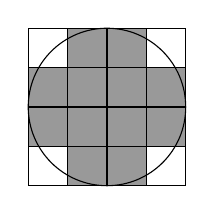
\begin{tikzpicture}[scale=0.5]
                % Draw the outer square
                \draw[black] (-2,-2) rectangle (2,2);
                % Draw filled squares inside the circle
                \foreach \x in {-1.5,-0.5,0.5,1.5}{
                \foreach \y in {-1.5,-0.5,0.5,1.5}{
                    % Calculate distance from center
                    \pgfmathparse{(\x)^2 + (\y)^2}
                    \ifdim \pgfmathresult pt < 4pt
                    % Fill the square
                    \filldraw[fill=black!40] (\x-0.5,\y-0.5) rectangle (\x+0.5,\y+0.5);
                    \fi
                };
                }
                % Draw the circle for reference
                \draw (0,0) circle (2cm);
            \end{tikzpicture}
            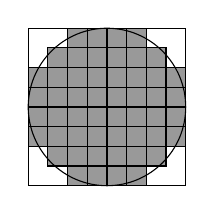
\begin{tikzpicture}[scale=0.5]
                % Draw the outer square
                \draw[black] (-2,-2) rectangle (2,2);
                % Draw filled squares inside the circle
                \foreach \x in {-1.75,-1.25,...,1.75}{
                \foreach \y in {-1.75,-1.25,...,1.75}{
                    \pgfmathparse{(\x)^2 + (\y)^2}
                    \ifdim \pgfmathresult pt < 4pt
                    \filldraw[fill=black!40] (\x-0.25,\y-0.25) rectangle (\x+0.25,\y+0.25);
                    \fi
                }
                }
                % Draw the circle for reference
                \draw (0,0) circle (2cm);
            \end{tikzpicture}
            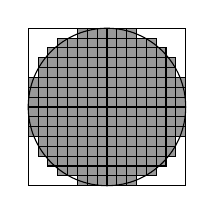
\begin{tikzpicture}[scale=0.5]
                % Draw the outer square
                \draw[black] (-2,-2) rectangle (2,2);
                % Draw filled squares inside the circle
                \foreach \x in {-1.875,-1.625,...,1.875}{
                \foreach \y in {-1.875,-1.625,...,1.875}{
                    \pgfmathparse{(\x)^2 + (\y)^2}
                    \ifdim \pgfmathresult pt < 4pt
                    \filldraw[fill=black!40] (\x-0.125,\y-0.125) rectangle (\x+0.125,\y+0.125);
                    \fi
                }
                }
                % Draw the circle for reference
                \draw (0,0) circle (2cm);
            \end{tikzpicture}
            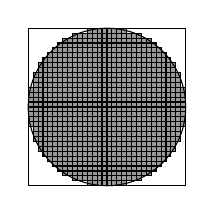
\begin{tikzpicture}[scale=0.5]
                % Draw the outer square
                \draw[black] (-2,-2) rectangle (2,2);
                % Draw filled squares inside the circle
                \foreach \x in {-1.9375,-1.8125,...,1.9375}{
                \foreach \y in {-1.9375,-1.8125,...,1.9375}{
                    \pgfmathparse{(\x)^2 + (\y)^2}
                    \ifdim \pgfmathresult pt < 4pt
                    \filldraw[fill=black!40] (\x-0.0625,\y-0.0625) rectangle (\x+0.0625,\y+0.0625);
                    \fi
                }
                }
                % Draw the circle for reference
                \draw (0,0) circle (2cm);
            \end{tikzpicture}
        \end{center}
        $\textbf{Proof of falseness.}$ We will call an $n-teselation$ a recurrent sequence in which we 
        double the amount of squares in the grid, and bound upperly the unitary
        circumference of an $(n-1)-teselation$ (the picture does not shows it, but the original puzzle does). 
        
        Let $(a_n)_{n=m}^{\infty}$ be defined as the side of any grid
        square in an $n-teselation$. 

        Let $(b_n)_{n=m}^{\infty}$ be defined as the amount of contact points
        between the shaded squares and the unitary circumference.
        
        We claim that $(a_n)$ converges. To prove this claim note that $\displaystyle (a_n) = \frac{L}{2^n} = L\frac{1}{2^n}$,
        which converges to zero.

        We also claim that $(b_n)$ does not converge. To prove this claim we note that $(b_n)$ is lowerly bounded by the sequence $(c_n) = n/4$, which does not converge.
        
        Assuming that for any n-teselation only squares are added, each one adjacent to the former ones, as $(a_n)$ converges, this means that the distance between (discrete distance, also known as taxist norm) each adjacent contact point
        decreases exponentially, and by triangle inequality, their euclidean distance decreases exponentially as well. This paragraph can be reduced to the inequality 
        \begin{center}
            $\displaystyle 2a_n \geq \sqrt{2}a_n$.
        \end{center}

        Let $C$ be the points of the circumference.
        We define the set $X := \{x \in C: x \text{ is a contact point}\}$, we aim to prove that there exist a point in $X$ that is not $\varepsilon$-adherent for some $\varepsilon > 0$ to some other point of $X$,
        this means that $X$ will not be dense, and will not define a proper perimeter.

        Let $c \in C$. Suppose, for the sake of contradiction, that there existed an n-teselation such that for any $q \in X$, for any $\varepsilon > 0$, the ball of center $c$ and radius $\varepsilon$ contains 
        $q$. I.e. $d(c,q) \leq \varepsilon$ (where $d()$ denotes euclidean distance), this would mean that $X$ is dense.
        
        Let $q_0, q_1$ be fixed points in $X$ such that $d(q_0,q_1) \leq \sqrt{2}a_n$, these points can be found since 
        for some n-teselation the euclidean distance between contact points converges to zero.
        Since $C$ is dense we can find $q_0 < c < q_1$.

        Let $3\varepsilon \leq \sqrt{2}a_n$. We have that 
        \begin{center}
            $\displaystyle d(q_0, c) + d(c, q_1) \geq d(q_0, q_1)$, so $\displaystyle 2\varepsilon \geq \sqrt{2}a_n$.
        \end{center}
        Hence $\displaystyle 3\varepsilon > 2\varepsilon \geq \sqrt{2}a_n$, which is a contradiction.
        \begin{flushright}
            \qed
        \end{flushright}
    \end{enumerate}
\end{document}